\begin{table}[h]
  \centering
  \begin{tabular}{|l|c|}
    \hline
    \textbf{Zastávka} & \# \\ \hline
    Lesná, Haškova & 0 \\ \hline
    Brechtova & 1 \\ \hline
    Blažkova & 2 \\ \hline
    Arbesova & 3 \\ \hline
    Heleny Malířové & 4 \\ \hline
    Lesná, nádraží & 5 \\ \hline
    Štefánikova čtvrť & 6 \\ \hline
    Provozníkova & 7 \\ \hline
    Lesnická & 9 \\ \hline
    Zemědělská & 10 \\ \hline
    Černá Pole, Erbenova & 11 \\ \hline
  \end{tabular}
  \caption{Rozpis zastávok}
\end{table}

\begin{table}[h]
  \centering
  \begin{tabular}{|c|l|}
    \hline
    \textbf{h} & \textbf{Odchody} \\ \hline
    05 & 00, 12, 24, 36, 48 \\ \hline
    06 & 00, 08, 17, 25, 34, 42, 51 \\ \hline
    07 & 00, 10, 20, 30, 40, 50 \\ \hline
    08 & 00, 12, 24, 36, 48 \\ \hline
    09 & 00, 08, 17, 25, 34, 42, 51 \\ \hline
    10 & 00, 10, 20, 30, 40, 50 \\ \hline
    11 & 00, 15, 30, 45 \\ \hline
    12 & 00, 12, 24, 36, 48 \\ \hline
    13 & 00, 12, 24, 36, 48 \\ \hline
    14 & 00, 07, 15, 22, 30, 37, 45, 52 \\ \hline
    15 & 00, 08, 17, 25, 34, 42, 51 \\ \hline
    16 & 00, 08, 17, 25, 34, 42, 51 \\ \hline
    17 & 00, 08, 17, 25, 34, 42, 51 \\ \hline
    18 & 00, 15, 30, 45 \\ \hline
    19 & 00, 20, 40 \\ \hline
    20 & 00, 12, 24, 36, 48 \\ \hline
    21 & 00, 15, 30, 45 \\ \hline
    22 & 00, 15, 30, 45 \\ \hline
  \end{tabular}
  \caption{Časový rozpis}
\end{table}

\begin{table}[h]
  \centering
  \begin{tabular}{|l|c|}
    \hline
    \textbf{Vstup} & \textbf{Hodnota} \\ \hline
    Kapacita vozidla & 160 \\ \hline
    Počet miest na sedenie & 60 \\ \hline
    Kompenzácia vozidla & 66.35 Kč \\ \hline
    Dĺžka trasy & 3.8 km \\ \hline
    Cena lístka & 25 Kč \\ \hline
  \end{tabular}
  \caption{Parametre vozidla a trasy}
\end{table}

\begin{table}[h]
  \centering
  \begin{tabular}{|l|c|}
    \hline
    \textbf{Výstup} & \textbf{Hodnota} \\ \hline
    Počet príchodov cestujúcich & 11790 \\ \hline
    Počet prevezených cestujúcich & 11790 \\ \hline
    Počet neobslúžených cestujúcich & 0 (0.0\,\%) \\ \hline
    Celkový čas strávený čakaním & 66008 min \\ \hline
    Priemerný čas strávený čakaním & 6 min \\ \hline
    Celková kompenzácia & -39937 Kč \\ \hline
    Celkový zisk & 254813 Kč \\ \hline
    Priemerná spokojnosť cestujúcich & 99.79\,\% \\ \hline
    Celkový počet vozidiel & 99 \\ \hline
    Priemerná naplnenosť vozidiel & 29 (18.07\,\%) \\ \hline
  \end{tabular}
  \caption{Výstupy simulácie}
\end{table}

\begin{figure}[h]
  \centering
  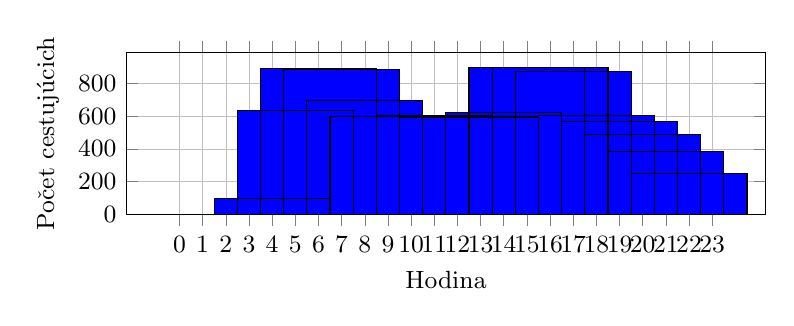
\begin{tikzpicture}
    \begin{axis}[
      width=0.8\textwidth,
      height=0.3\textwidth,
      xlabel={Hodina},
      ylabel={Počet cestujúcich},
      ymin=0,
      xtick={0,1,...,23},
      grid=both,
      major grid style={line width=.2pt,draw=gray!50},
      minor grid style={line width=.1pt,draw=gray!20},
      tick label style={font=\small},
      label style={font=\small},
      legend style={font=\small, at={(0.5,-0.2)}, anchor=north, legend columns=-1},
      ybar,
      bar width=5,
      ]
      \addplot[fill=blue] coordinates {
        (0, 0) (1, 0) (2, 0) (3, 0) (4, 99) (5, 637) (6, 894) (7, 887) 
        (8, 694) (9, 598) (10, 599) (11, 604) (12, 594) (13, 595) 
        (14, 624) (15, 899) (16, 899) (17, 873) (18, 602) (19, 570) 
        (20, 489) (21, 384) (22, 249) (23, 0)
      };
    \end{axis}
  \end{tikzpicture}
  \caption{Počet cestujúcich prichádzajúcich na zastávku za hodinu}
\end{figure}

\begin{figure}[h]
  \centering
  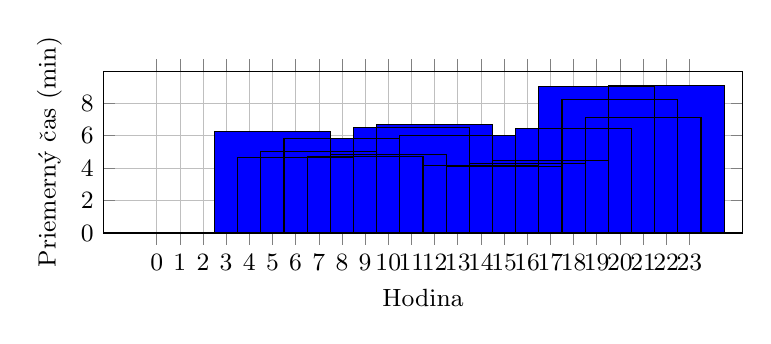
\begin{tikzpicture}
    \begin{axis}[
      width=0.8\textwidth,
      height=0.3\textwidth,
      xlabel={Hodina},
      ylabel={Priemerný čas (min)},
      ymin=0,
      xtick={0,1,...,23},
      grid=both,
      major grid style={line width=.2pt,draw=gray!50},
      minor grid style={line width=.1pt,draw=gray!20},
      tick label style={font=\small},
      label style={font=\small},
      legend style={font=\small, at={(0.5,-0.2)}, anchor=north, legend columns=-1},
      ybar,
      bar width=5,
      ]
      \addplot[fill=blue] coordinates {
        (0, 0) (1, 0) (2, 0) (3, 0) (4, 0) (5, 6.279434850863423) (6, 4.668903803131991) 
        (7, 5.00901916572717) (8, 5.845821325648415) (9, 4.724080267558528) 
        (10, 4.856427378964941) (11, 6.533112582781457) (12, 6.683501683501683) 
        (13, 5.994957983193277) (14, 4.174679487179487) (15, 4.0945494994438265) 
        (16, 4.303670745272525) (17, 4.497136311569301) (18, 6.423588039867109) 
        (19, 9.033333333333333) (20, 8.210633946830265) (21, 7.145833333333333) 
        (22, 9.080321285140561) (23, 0)
      };
    \end{axis}
  \end{tikzpicture}
  \caption{Priemerný čas strávený čakaním za hodinu}
\end{figure}

\begin{figure}[h]
  \centering
  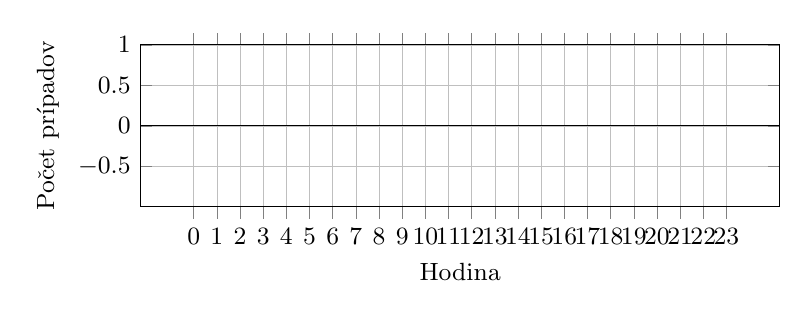
\begin{tikzpicture}
    \begin{axis}[
      width=0.8\textwidth,
      height=0.3\textwidth,
      xlabel={Hodina},
      ylabel={Počet prípadov},
      ymin=0,
      xtick={0,1,...,23},
      grid=both,
      major grid style={line width=.2pt,draw=gray!50},
      minor grid style={line width=.1pt,draw=gray!20},
      tick label style={font=\small},
      label style={font=\small},
      legend style={font=\small, at={(0.5,-0.2)}, anchor=north, legend columns=-1},
      ybar,
      bar width=5,
      ]
      \addplot[fill=blue] coordinates {
        (0, 0) (1, 0) (2, 0) (3, 0) (4, 0) (5, 0) (6, 0) (7, 0) 
        (8, 0) (9, 0) (10, 0) (11, 0) (12, 0) (13, 0) 
        (14, 0) (15, 0) (16, 0) (17, 0) (18, 0) (19, 0) 
        (20, 0) (21, 0) (22, 0) (23, 0)
      };
    \end{axis}
  \end{tikzpicture}
  \caption{Počet prípadov, kedy sa cestujúci nezmestili do vozidla za hodinu}
\end{figure}